\documentclass[9pt,pdf,hyperref={unicode}]{beamer}
\beamertemplatenavigationsymbolsempty

\setbeamertemplate{blocks}[rounded=true, shadow=true]
\setbeamertemplate{footline}[page number]
\usepackage{multicol}

\usefonttheme{serif}

\usepackage[utf8]{inputenc}
\usepackage[english, russian]{babel}
\usepackage{amsmath,mathrsfs,mathtext}
\usepackage{graphicx, epsfig}
\usepackage{caption}
\usepackage{subfig}
\usepackage{amsmath, bm}

\usepackage{comment}
\usepackage{autonum}
\usepackage{tabularx}

\usepackage{tikz}
\newcommand{\bmatr}{{\mathbf{B}}}
\newcommand{\cmatr}{{\mathbf{C}}}
\newcommand{\hmatr}{{\mathbf{H}}}
\newcommand{\fmatr}{{\mathbf{F}}}
\newcommand{\mmatr}{{\mathbf{M}}}
\newcommand{\xmatr}{{\mathbf{X}}}
\newcommand{\pmatr}{{\mathbf{P}}}
\newcommand{\xmatrt}{{\tilde{\mathbf{X}}}}
\newcommand{\imatr}{{\mathbf{I}}}
\newcommand{\vmatr}{{\mathbf{V}}}
\newcommand{\wmatr}{{\mathbf{W}}}
\newcommand{\umatr}{{\mathbf{U}}}
\newcommand{\zmatr}{{\mathbf{Z}}}
\newcommand{\zmatrt}{{\tilde{\mathbf{Z}}}}
\newcommand{\Tmatr}{\mathbf{T}}
\newcommand{\lambdamatr}{{\mathbf{\Lambda}}}
\newcommand{\phimatr}{\mathbf{\Phi}}
\newcommand{\sigmamatr}{\mathbf{\Sigma}}
\newcommand{\thetamatr}{\boldsymbol{\Theta}}
\newcommand{\Ri}{\mathcal{R}}
\newcommand{\rk}{\mathfrak{r}}
\newcommand{\ab}{{\wm}}
\newcommand{\bb}{{\mathbf{b}}}
\newcommand{\cb}{{\mathbf{c}}}
\newcommand{\db}{{\mathbf{d}}}
\newcommand{\eb}{{\mathbf{e}}}
\newcommand{\fb}{{\mathbf{f}}}
\newcommand{\gb}{{\mathbf{g}}}
\newcommand{\hb}{{\mathbf{h}}}
\newcommand{\mb}{{\mathbf{m}}}
\newcommand{\pb}{{\mathbf{p}}}
\newcommand{\qb}{{\mathbf{q}}}
\newcommand{\rb}{{\mathbf{r}}}
\newcommand{\tb}{{\mathbf{t}}}
\newcommand{\ub}{{\mathbf{u}}}
\newcommand{\vb}{{\mathbf{v}}}
\newcommand{\wb}{{\mathbf{W}}}
\newcommand{\xb}{{\mathbf{x}}}
\newcommand{\xt}{{\tilde{x}}}
\newcommand{\xbt}{\tilde{{\mathbf{x}}}}
\newcommand{\yb}{{\mathbf{y}}}
\newcommand{\zb}{{\mathbf{z}}}
\newcommand{\zt}{{\tilde{z}}}
\newcommand{\zbt}{{\tilde{\mathbf{z}}}}
\newcommand{\mub}{{\boldsymbol{\mu}}}
\newcommand{\alphab}{{\boldsymbol{\alpha}}}
\newcommand{\thetab}{{\boldsymbol{\theta}}}
\newcommand{\iotab}{\boldsymbol{\iota}}
\newcommand{\zetab}{\boldsymbol{\zeta}}
\newcommand{\xib}{\boldsymbol{\xi}}
\newcommand{\xibt}{\tilde{\boldsymbol{\xi}}}
\newcommand{\xit}{\tilde{\xi}}
\newcommand{\betab}{{\boldsymbol{\beta}}}
\newcommand{\phib}{{\boldsymbol{\phi}}}
\newcommand{\psib}{{\boldsymbol{\psi}}}
\newcommand{\gammab}{{\boldsymbol{\gamma}}}
\newcommand{\lambdab}{{\boldsymbol{\lambda}}}
\newcommand{\varepsilonb}{{\boldsymbol{\varepsilon}}}
\newcommand{\pib}{{\boldsymbol{\pi}}}
\newcommand{\sigmab}{{\boldsymbol{\sigma}}}




\newcommand{\scl}{s_{\mathsf{c}}}
\newcommand{\shi}{s_{\mathsf{h}}}
\newcommand{\shib}{\mathbf{s}_{\mathsf{h}}}
\newcommand{\MOD}{M}
\newcommand{\entr}{\mathsf{H}}
\newcommand{\REG}{\Omega}
\newcommand{\Mquol}{V}
\newcommand{\prob}{p}
\newcommand{\expec}{\mathsf{E}}

\newcommand{\xo}{{\overline{x}}}
\newcommand{\Xo}{{\overline{x}}}
\newcommand{\yo}{{\overline{y}}}

\newcommand{\xbo}{{\overline{\mathbf{x}}}}
\newcommand{\Xbo}{{\overline{\mathbf{X}}}}

\newcommand{\Amc}{{\mathcal{A}}}
\newcommand{\Bmc}{{\mathcal{B}}}
\newcommand{\Cmc}{{\mathcal{C}}}
\newcommand{\Jmc}{{\mathcal{J}}}
\newcommand{\Imc}{{\mathcal{I}}}
\newcommand{\Kmc}{{\mathcal{K}}}
\newcommand{\Lmc}{{\mathcal{L}}}
\newcommand{\Mmc}{{\mathcal{M}}}
\newcommand{\Nmc}{{\mathcal{N}}}
\newcommand{\Pmc}{{\mathcal{P}}}
\newcommand{\Tmc}{{\mathcal{T}}}
\newcommand{\Vmc}{{\mathcal{V}}}
\newcommand{\Wmc}{{\mathcal{W}}}
\newcommand{\Smi}{{\mathcal{S}}}

\newcommand{\T}{^{\text{\tiny\sffamily\upshape\mdseries T}}}
\newcommand{\deist}{\mathbb{R}}
\newcommand{\ebb}{\mathbb{E}}

\newcommand{\Amatr}{\wm}
\newcommand{\X}{\mathbf{X}}
\newcommand{\Z}{\mathbf{Z}}
\newcommand{\Umatr}{\mathbf{U}}
\newcommand{\zetavec}{\boldsymbol{\zeta}}

\newcommand{\M}{\mathbf{M}}
\newcommand{\x}{{\mathbf{x}}}
\newcommand{\z}{{\mathbf{z}}}
\newcommand{\ical}{{\mathcal{I}}}
\newcommand{\tvec}{{\mathbf{t}}}
\newcommand{\xvec}{{\mathbf{x}}}
\newcommand{\zvec}{{\mathbf{z}}}
\newcommand{\bvec}{{\mathbf{b}}}
\newcommand{\qvec}{{\mathbf{z}}}
\newcommand{\pvec}{{\mathbf{p}}}
\newcommand{\wvec}{{\mathbf{W}}}
\newcommand{\rvec}{{\mathbf{r}}}
\newcommand{\thetavec}{{\mathbf{\theta}}}
\newcommand{\y}{{\mathbf{y}}}
\newcommand{\g}{{\mathbf{g}}}
\newcommand{\w}{{\mathbf{W}}}
\newcommand{\wm}{{\mathbf{w}}}
\newcommand{\m}{{\mathbf{m}}}

\usetheme{Warsaw}%{Singapore}%{Warsaw}%{Warsaw}%{Darmstadt}
\usecolortheme{sidebartab}
\definecolor{beamer@blendedblue}{RGB}{15,120,80}
%----------------------------------------------------------------------------------------------------------
\title[\hbox to 56mm{Аддитивная регуляризация  \hfill\insertframenumber\,/\,\inserttotalframenumber}]
{Аддитивная регуляризация и ее метапараметры при выборе структуры сетей глубокого обучения}
\author[К.\,О. Вайсер ]{\large \\Кирилл Олегович Вайсер}
\institute{\large
Московский физико-технический институт}

\date{\footnotesize{\emph{Курс:} Численные методы обучения по прецедентам\par (практика, В.\,В. Стрижов)/Группа 774, весна 2020}\\\footnotesize{\emph{Консультант:} аспирант М.\ С. Потанин}\\
\footnotesize{\emph{Научный руководитель:} д.ф.-м.н. В.\ В. Стрижов}}
%----------------------------------------------------------------------------------------------------------
\begin{document}
%----------------------------------------------------------------------------------------------------------
\begin{frame}
%\thispagestyle{empty}
\titlepage
\end{frame}
%-----------------------------------------------------------------------------------------------------
\begin{frame}{Задача построения модели глубокого обучения}
\begin{block}{Цель работы}
Предложить метод построения критерия качества модели, учитывающего ее точность, сложность и устойчивость. Построить модель, удовлетворяющую этому критерию. 
\end{block}
\begin{block}{Проблема}
Нейронные сети, обладающие большой точностью, обычно демонстрируют высокую сложность и низкую устойчивость.
\end{block}
\begin{block}{Метод решения}
Построить функцию ошибки, включающую аддитивную регуляризацию.
\end{block}
\end{frame}
%----------------------------------------------------------------------------------------------------------
\begin{frame}{Постановка задачи}

Задана выборка, конечное множество пар  $$
(\mathbf{x},y) \in D,\quad \mathbf{x} \in \mathbb{R}^{n},\quad y\in \mathbb{R}.
$$
Структура модели имеет следующий вид
\begin{equation}
f = \sigma_k\circ\underset{1\times1}{\wm_k^\mathsf{T}\sigmab_{k-1}}\circ\w_{k-1}\sigmab_{k-2}\circ\dots\circ\underset{n_2 \times 1}{\w_2\sigmab_1}\circ\underset{n_1 \times n}{\w_1}\underset{n \times 1}{\x}.
\end{equation}
Функция ошибки имеет вид
\begin{equation}
L = \lambda_xE_{\mathbf{x}} + \lambda_yE_{\y} + \lambda_1\mathcal{R}_1+\dots+\lambda_k\mathcal{R}_k = \lambda_xE_x + \lambda_yE_y + \sum\limits_{i = 1}^k\mathbb{\lambda}_i \mathcal{R}_i(\mathbf{W}),
\end{equation}
где $\mathcal{R}_i = \mathcal{R}(\mathbf{W}) = [\rk_1(\mathbf{W}), \cdots , \rk_r(\mathbf{W})]^{\T}$~---вектор, состоящий из значений регуляризаторов $i$-ого слоя.
\\ Требуется решить задачу
\begin{equation}\label{eq:criterion_argmin}
\begin{array}{r@{}l}
\wm= \arg \min L(f| \mathbf{\lambda}),\\
\mathbf{\lambda }= \argmin L(f| \wm), \\
\end{array}
\end{equation}
при условии минимизации дисперсии параметров и сложности модели.
\begin{equation}
    \sum\limits_{i=1}^k \frac{1}{|W_k|}W_k^\mathsf{T}W_k \rightarrow \min, \quad \quad
    \sum\limits_{i=1}^k |W_k| \rightarrow \min.
\end{equation}
\end{frame}
%----------------------------------------------------------------------------------------------------------
%----------------------------------------------------------------------------------------------------------
\begin{frame}{Использование аддитивной регуляризации}
\begin{block}{Задание критерия качества}
    Вводится понятие сложности, устойчивости и точности модели.
\end{block}
\begin{block}{Построение критерия качества}
    Предлагается построить функцию ошибки, включающей аддитивную регуляризацию. Задаются гиперпараметры модели и метапараметры аддитивной регуляризации.
\end{block}
\begin{block}{Расписание оптимизации}
    Метапараметры оптимизации изменяются с течением итераций обучения сети. Порядок и правило их изменения задается экспертно.
\end{block}


\end{frame}
\begin{frame}{Критерии качества модели}
\begin{block}{Свойства модели}
    \begin{itemize}
    \item
    Сложность~---мера множества допустимых значений параметров модели
    $$
    \sum\limits_{i=1}^k |W_k|.$$
    \item
    Устойчивость~--- дисперсия ошибки и параметров
    $$
    \sum\limits_{i=1}^k \frac{1}{|W_k|}W_k^\mathsf{T}W_k.$$ 
    \item 
    Точность~---качество аппроксимации, выражаемое через значение функции ошибки $$\sum_{i = 1} ^ l (f(x_i) - y_i)^2. $$
\end{itemize}
\end{block}


\end{frame}
%----------------------------------------------------------------------------------------------------------
\begin{frame}{Каталог регуляризаторов аддитивной функции ошибки}
\begin{table}[h!]
\begin{center}
\begin{tabular}{|c|c|}
\hline
   Роль в аддитивной регуляризации & Тип регуляризатора  \\
  \hline
  \begin{flushleft}
  Ошибка выхода нейронной сети
  \end{flushleft} & $||\mathbf{y} - f(\w)||^2_2 $   \\
  \hline
  \begin{flushleft}
  Ошибка восстановления на каждом слое \end{flushleft} & $||\xb-\mathbf{r}(\xb)||^2_2$ \\
  \hline
  \begin{flushleft}
  $L_1$ и $L_2$ регуляризация \end{flushleft} & $||\wm-\wm_0||_1$, $||\wm-\wm_0||^2_2$ \\
  \hline 
  \begin{tabular}{c}
  \begin{flushleft}
       Штраф за отличие матрицы одного слоя\end{flushleft} \\ \begin{flushleft}
       от тождественного преобразования
       \end{flushleft}
  \end{tabular}

   & $||\w-\mathbf{I}||$  \\
  \hline
  \begin{flushleft}
  \begin{tabular}{c}
  
       Штраф за отличие матрицы одного слоя\\
       от метода главных компонент
       
  \end{tabular}
  \end{flushleft}
  & $||\w\w^T-\mathbf{I}||$ \\
  \hline
  \begin{flushleft}
  Тихоновская регуляризация \end{flushleft} & 
  $\|\mathbf{T}\w\|^2$  \\
  \hline
\end{tabular}
\end{center}
\end{table}
\end{frame}


%----------------------------------------------------------------------------------------------------------
\begin{frame}{Пример расписания регуляризации}
\begin{center}
\begin{figure}[h!]
\center{\includegraphics[width=\linewidth]{Opt_Schedule_1.png}}

\label{fig:opt schedule 1}
\end{figure}
Экспертное задание расписания оптимизации, первое расписание.
\end{center}
\end{frame}

%----------------------------------------------------------------------------------------------------------
\begin{frame}{Пример расписания регуляризации}
\begin{center}
\begin{figure}[h!]
\center{\includegraphics[width=\linewidth]{Opt_Schedule_2.png}}

\label{fig:opt schedule 2}
\end{figure}
Экспертное задание расписания оптимизации, второе расписание.
\end{center}
\end{frame}
%----------------------------------------------------------------------------------------------------------

\begin{frame}{Вычислительный эксперимент}
\begin{block}{Цель эксперимента}
    \begin{itemize}
        \item Проверить работоспособность предложенного метода и его соответствие целям исследования.
        \item Продемонстрировать эффект от использования аддитивной регуляризации
    \end{itemize}
\end{block}
\begin{center}
   Описание выборок для экспериментов.
\end{center}
\begin{table}[!htbp]
\captionsetup{justification=raggedright,singlelinecheck=false}
\label{table1}

\footnotesize
\begin{center}
\centering
\begin{tabular}{ | c | c | c |c | c | c | c | }
\hline
Выборка $\mathfrak{D}$ & Размер train  & Размер val  & Размер test& Объекты & Признаки\\
\hline
Credit Card & 18000 & 6000& 6000 & 30000 & 35  \\
\hline
Protein & 27438 & 9146 & 9146 & 45730 & 9 \\
\hline
Airbnb & 6298 & 2100 & 2100 & 10498 & 16 \\
\hline
Wine quality & 2938 & 980 & 980 & 4898 & 11 \\
\hline
Synthetic & 1200 & 400 & 400 & 2000 & 30 \\
\hline
\end{tabular}
\end{center}
\end{table}

\end{frame}


%----------------------------------------------------------------------------------------------------------
\begin{frame}{Дисперсия параметров во время обучения}
\begin{center}
Конфигурация : 4 слоя сети, 1 слой автоенкодера, 7 нейронов на каждый слой.
\begin{figure}[h!]
\center{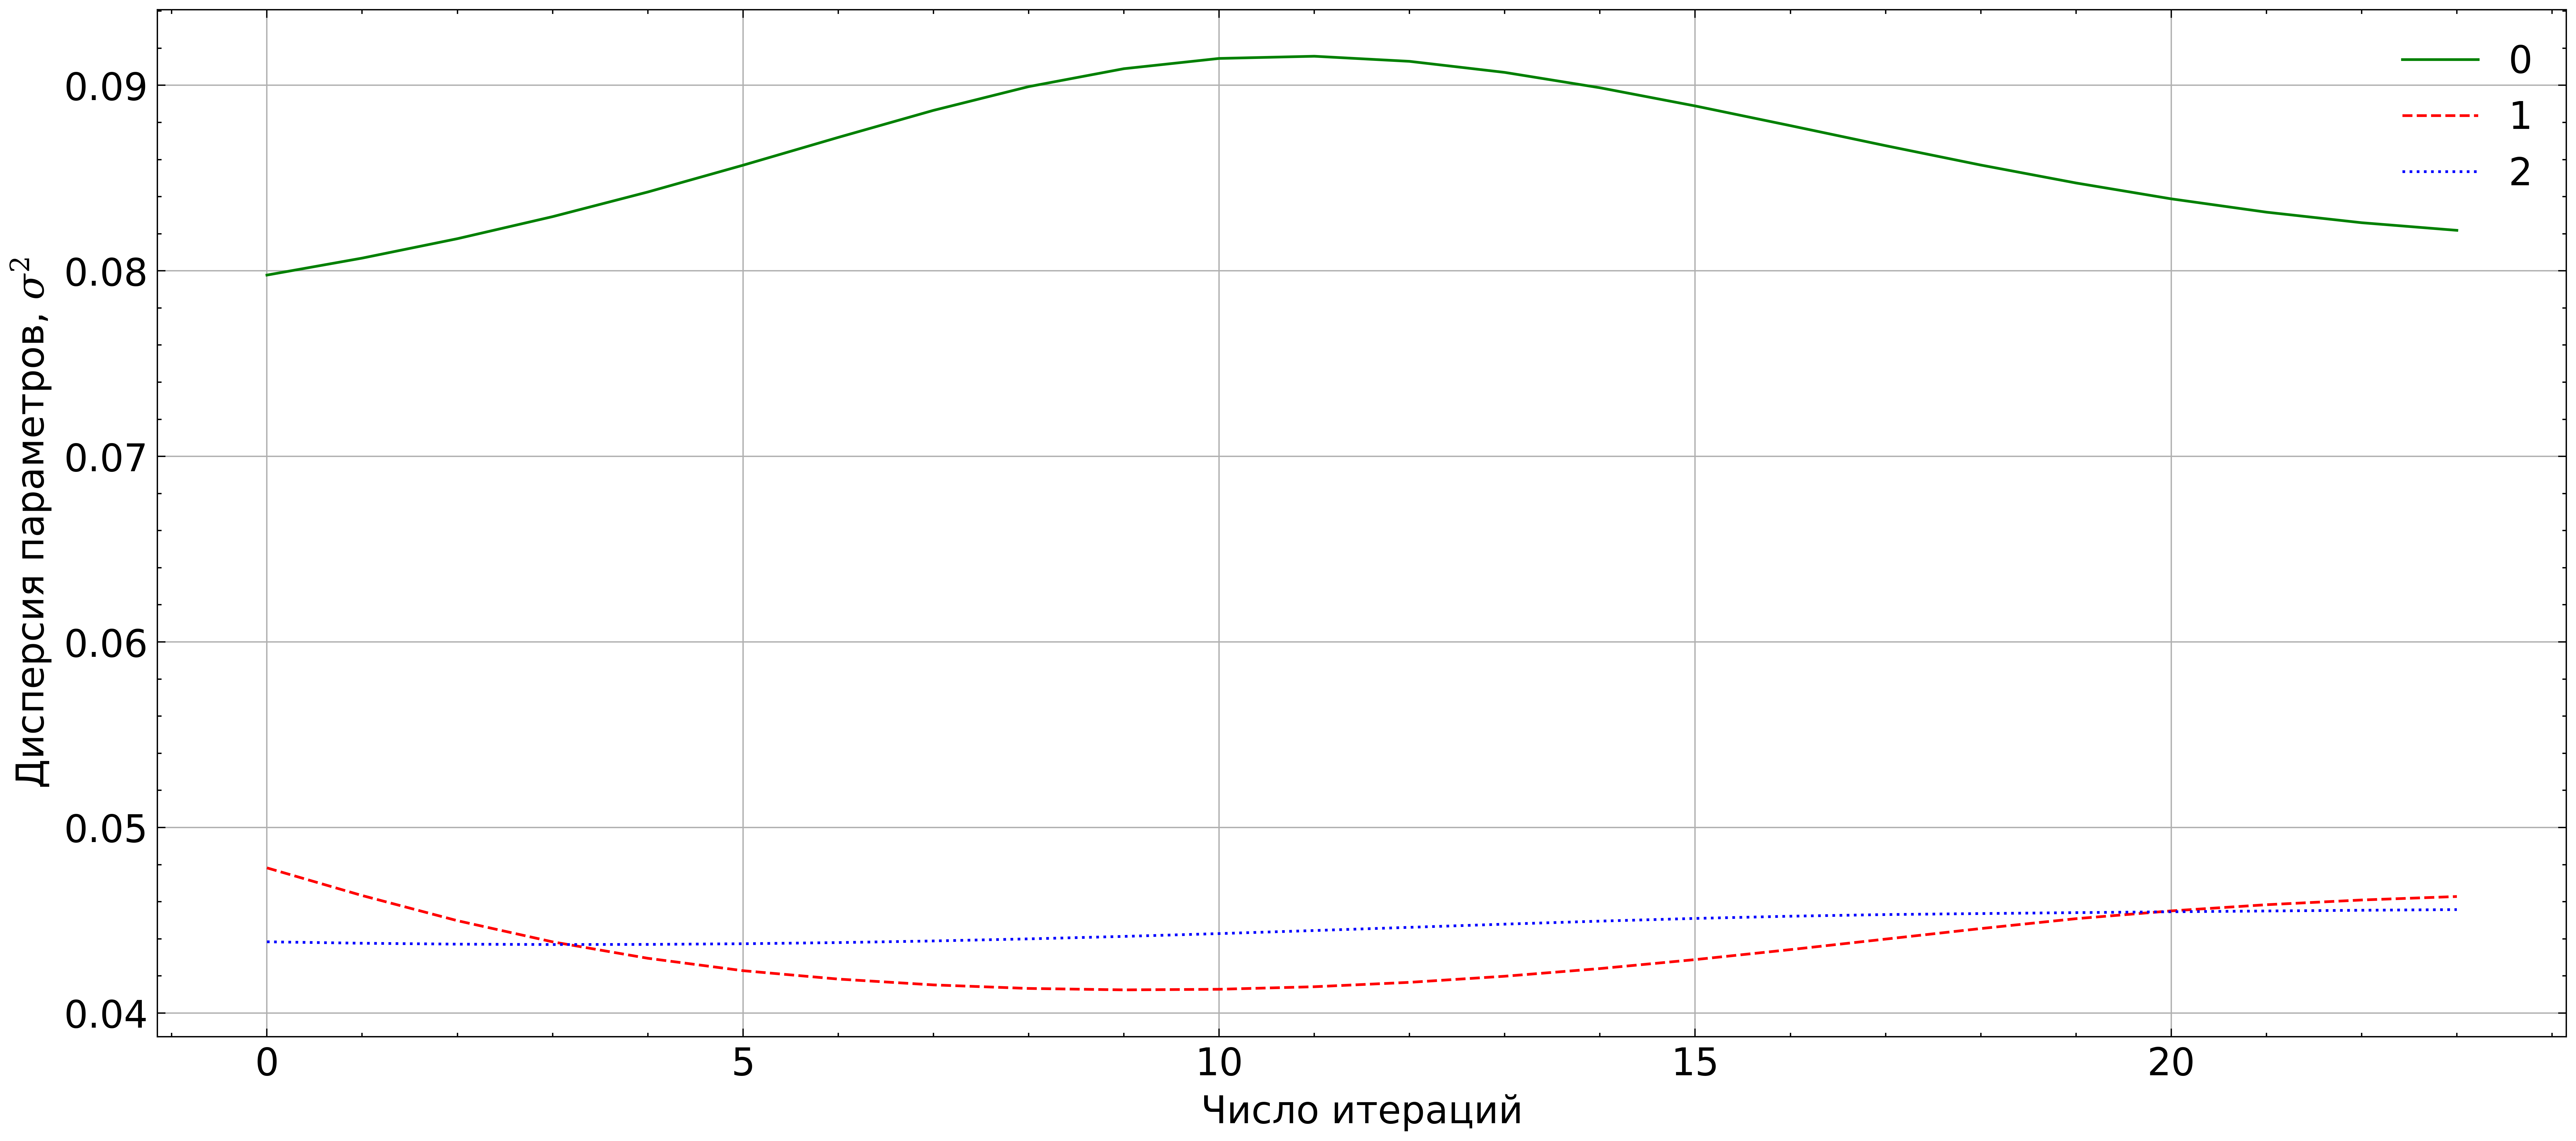
\includegraphics[width=\linewidth]{reg_under.png}}
\label{fig:opt schedule 2}
\end{figure}
За счет регуляризации модель становится более устойчивой, поэтому дисперсия параметров у регуляризованных решений меньше.
\end{center}
\end{frame}
%----------------------------------------------------------------------------------------------------------
\begin{frame}{Дисперсия параметров во время обучения}
\begin{center}
Конфигурация : 6 слоев сети, 1 слой автоенкодера, 9 нейронов на каждый слой.
\begin{figure}[h!]
\center{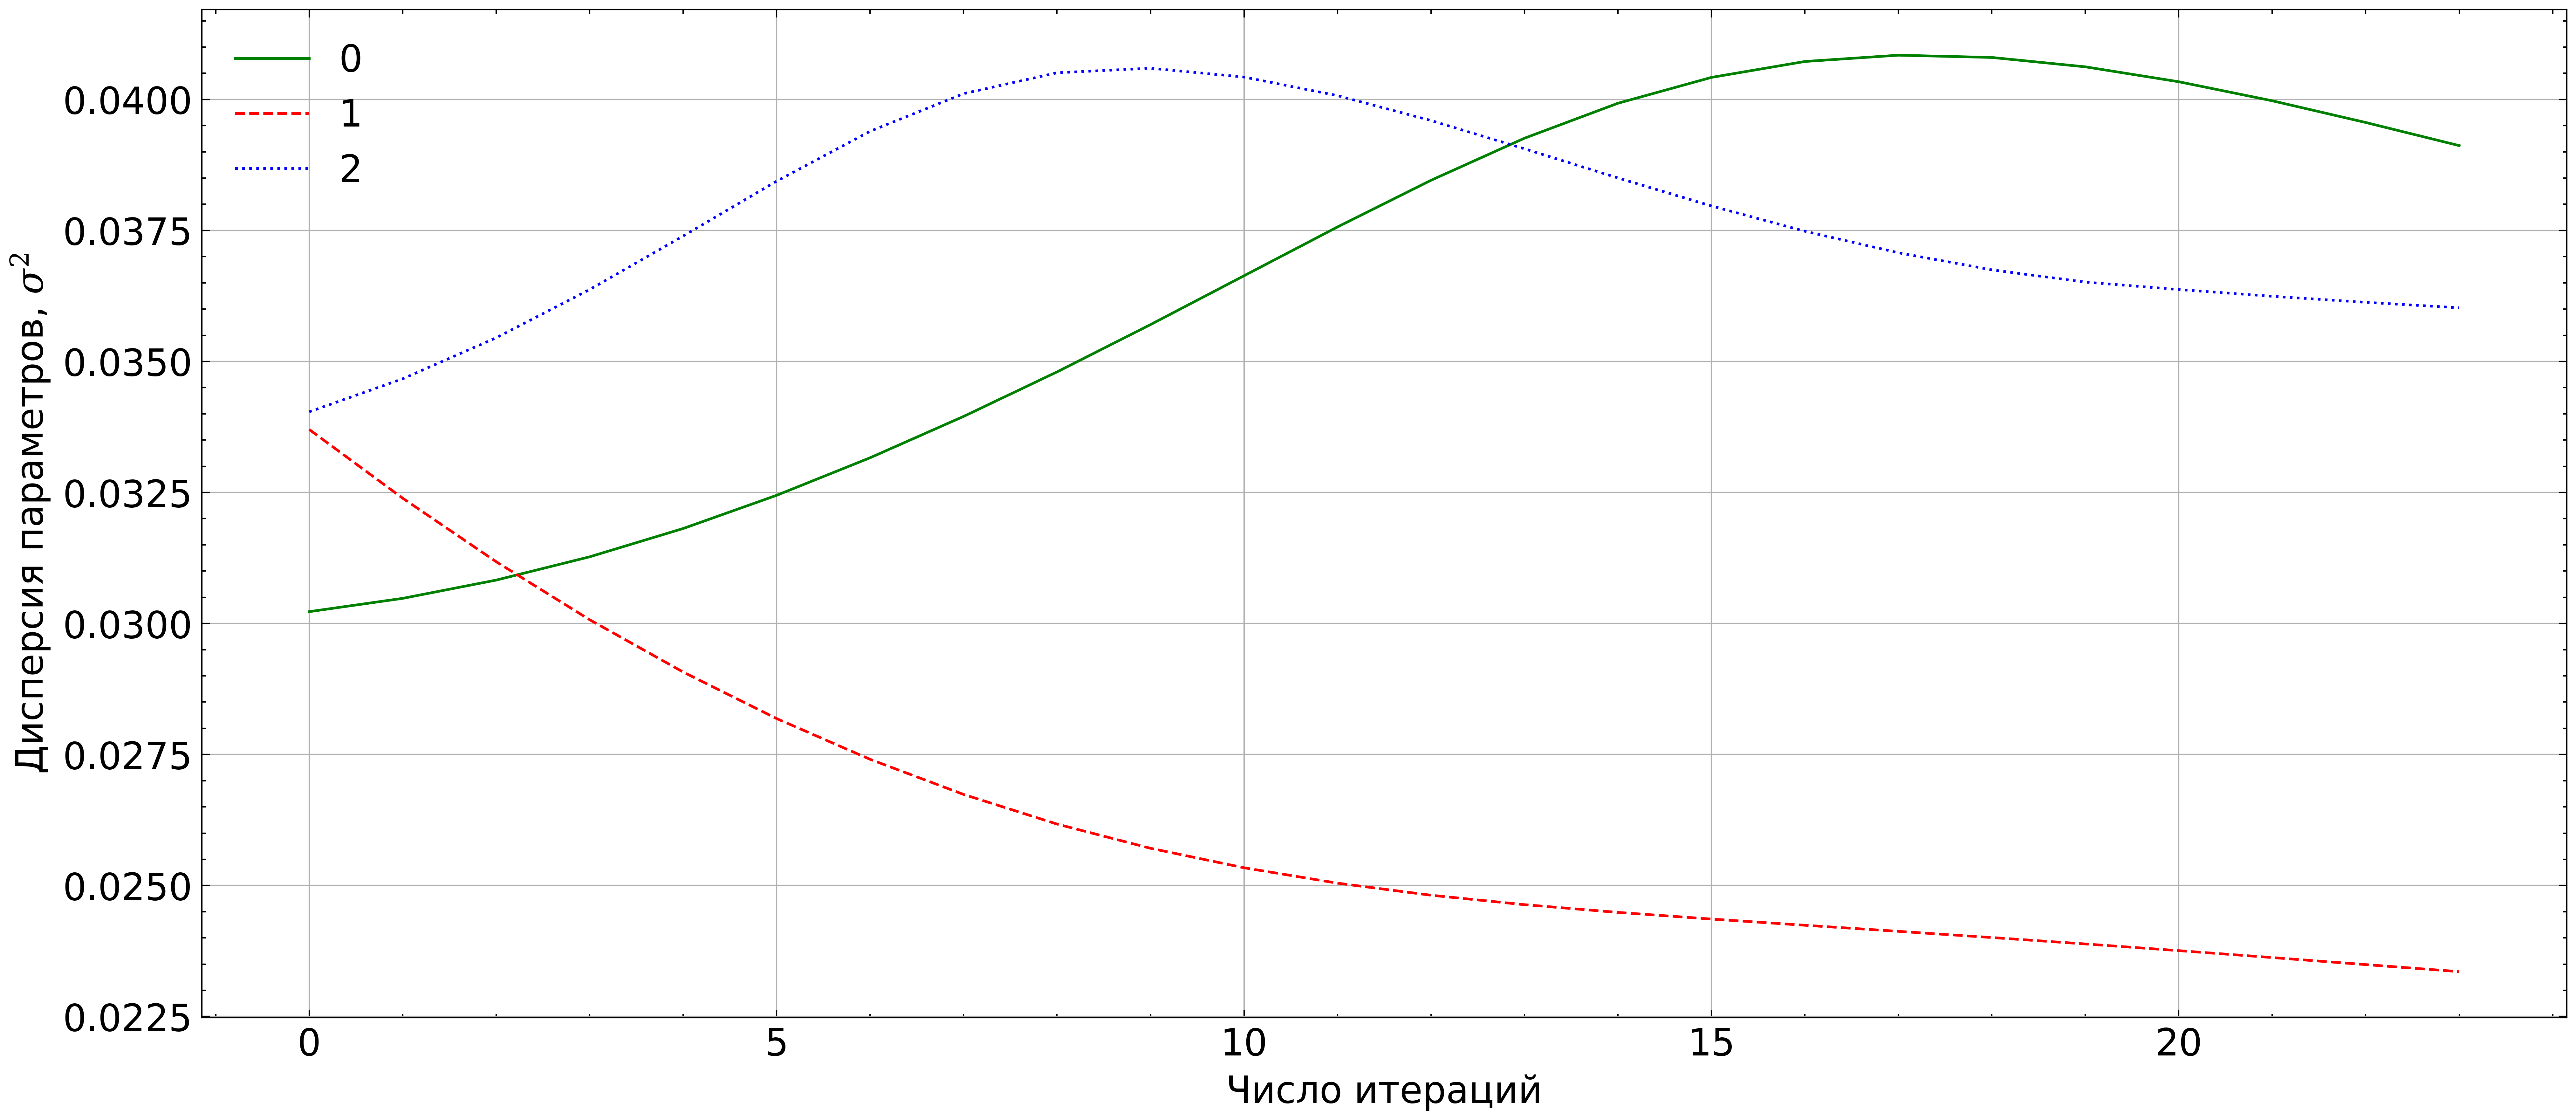
\includegraphics[width=\linewidth]{red_under.png}}

\label{fig:opt schedule 2}
\end{figure}
Первое расписание оптимизации демонстрирует большую эффективность, чем второе.
\end{center}
\end{frame}
%----------------------------------------------------------------------------------------------------------
\begin{frame}{Дисперсия параметров во время обучения}
\begin{center}
Конфигурация : 6 слоев сети, 4 слоя автоенкодера, 8 нейронов на каждый слой.
\begin{figure}[h!]
\center{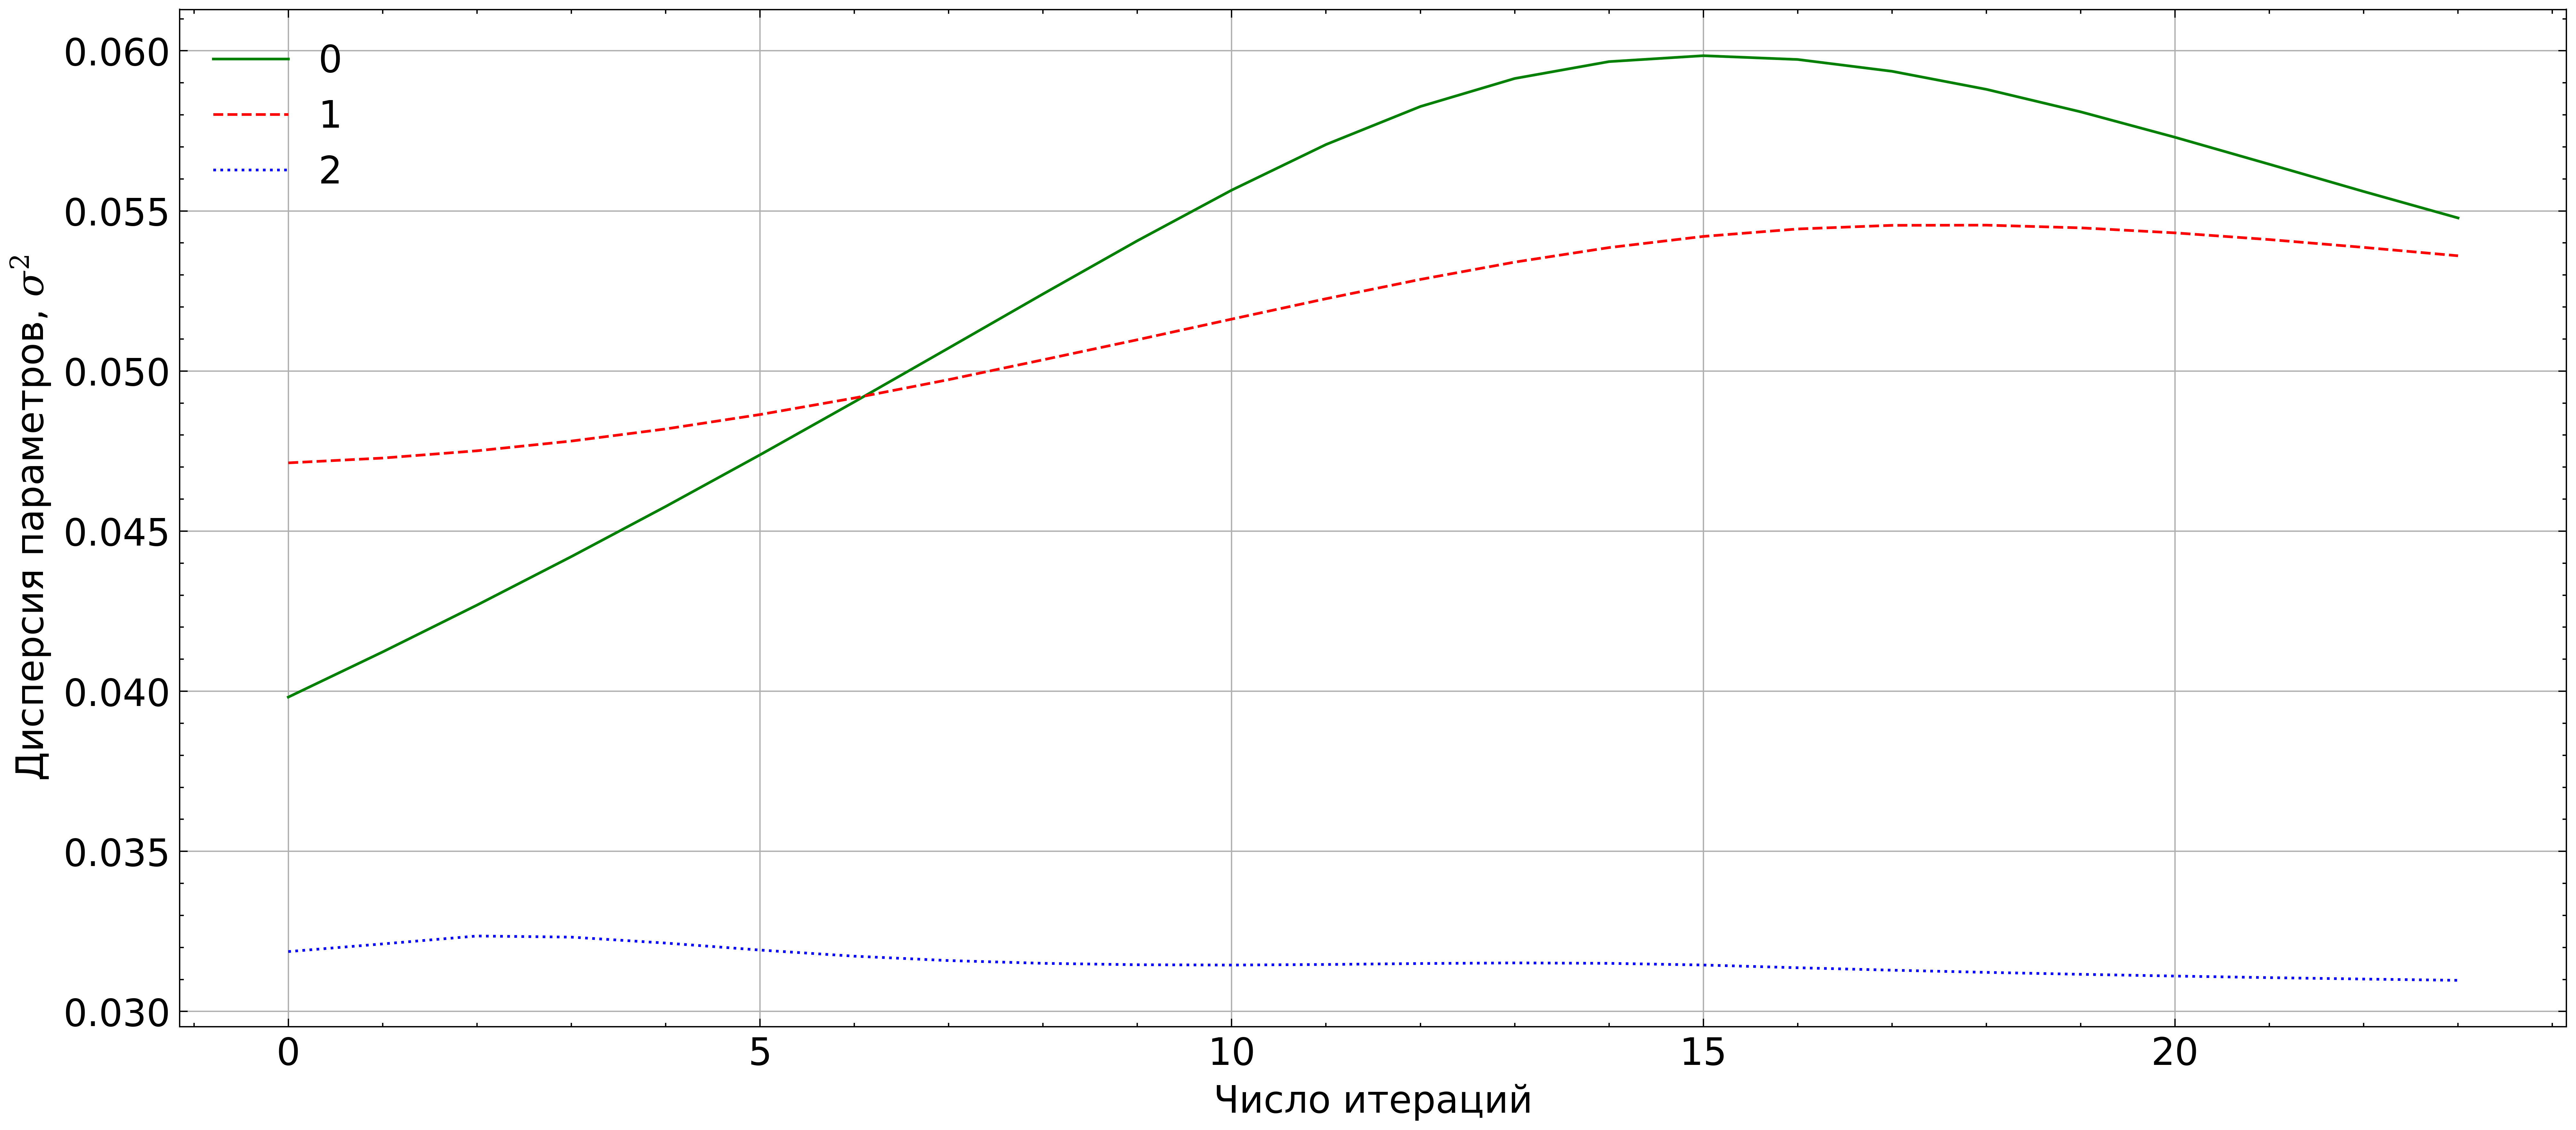
\includegraphics[width=\linewidth]{blue_under.png}}
\label{fig:opt schedule 2}
\end{figure}
Второе расписание оптимизации демонстрирует большую эффективность, чем первое.
\end{center}
\end{frame}
%----------------------------------------------------------------------------------------------------------
\begin{frame}{Зависимость точности от сложности}
\begin{center}
\begin{figure}[h!]
\center{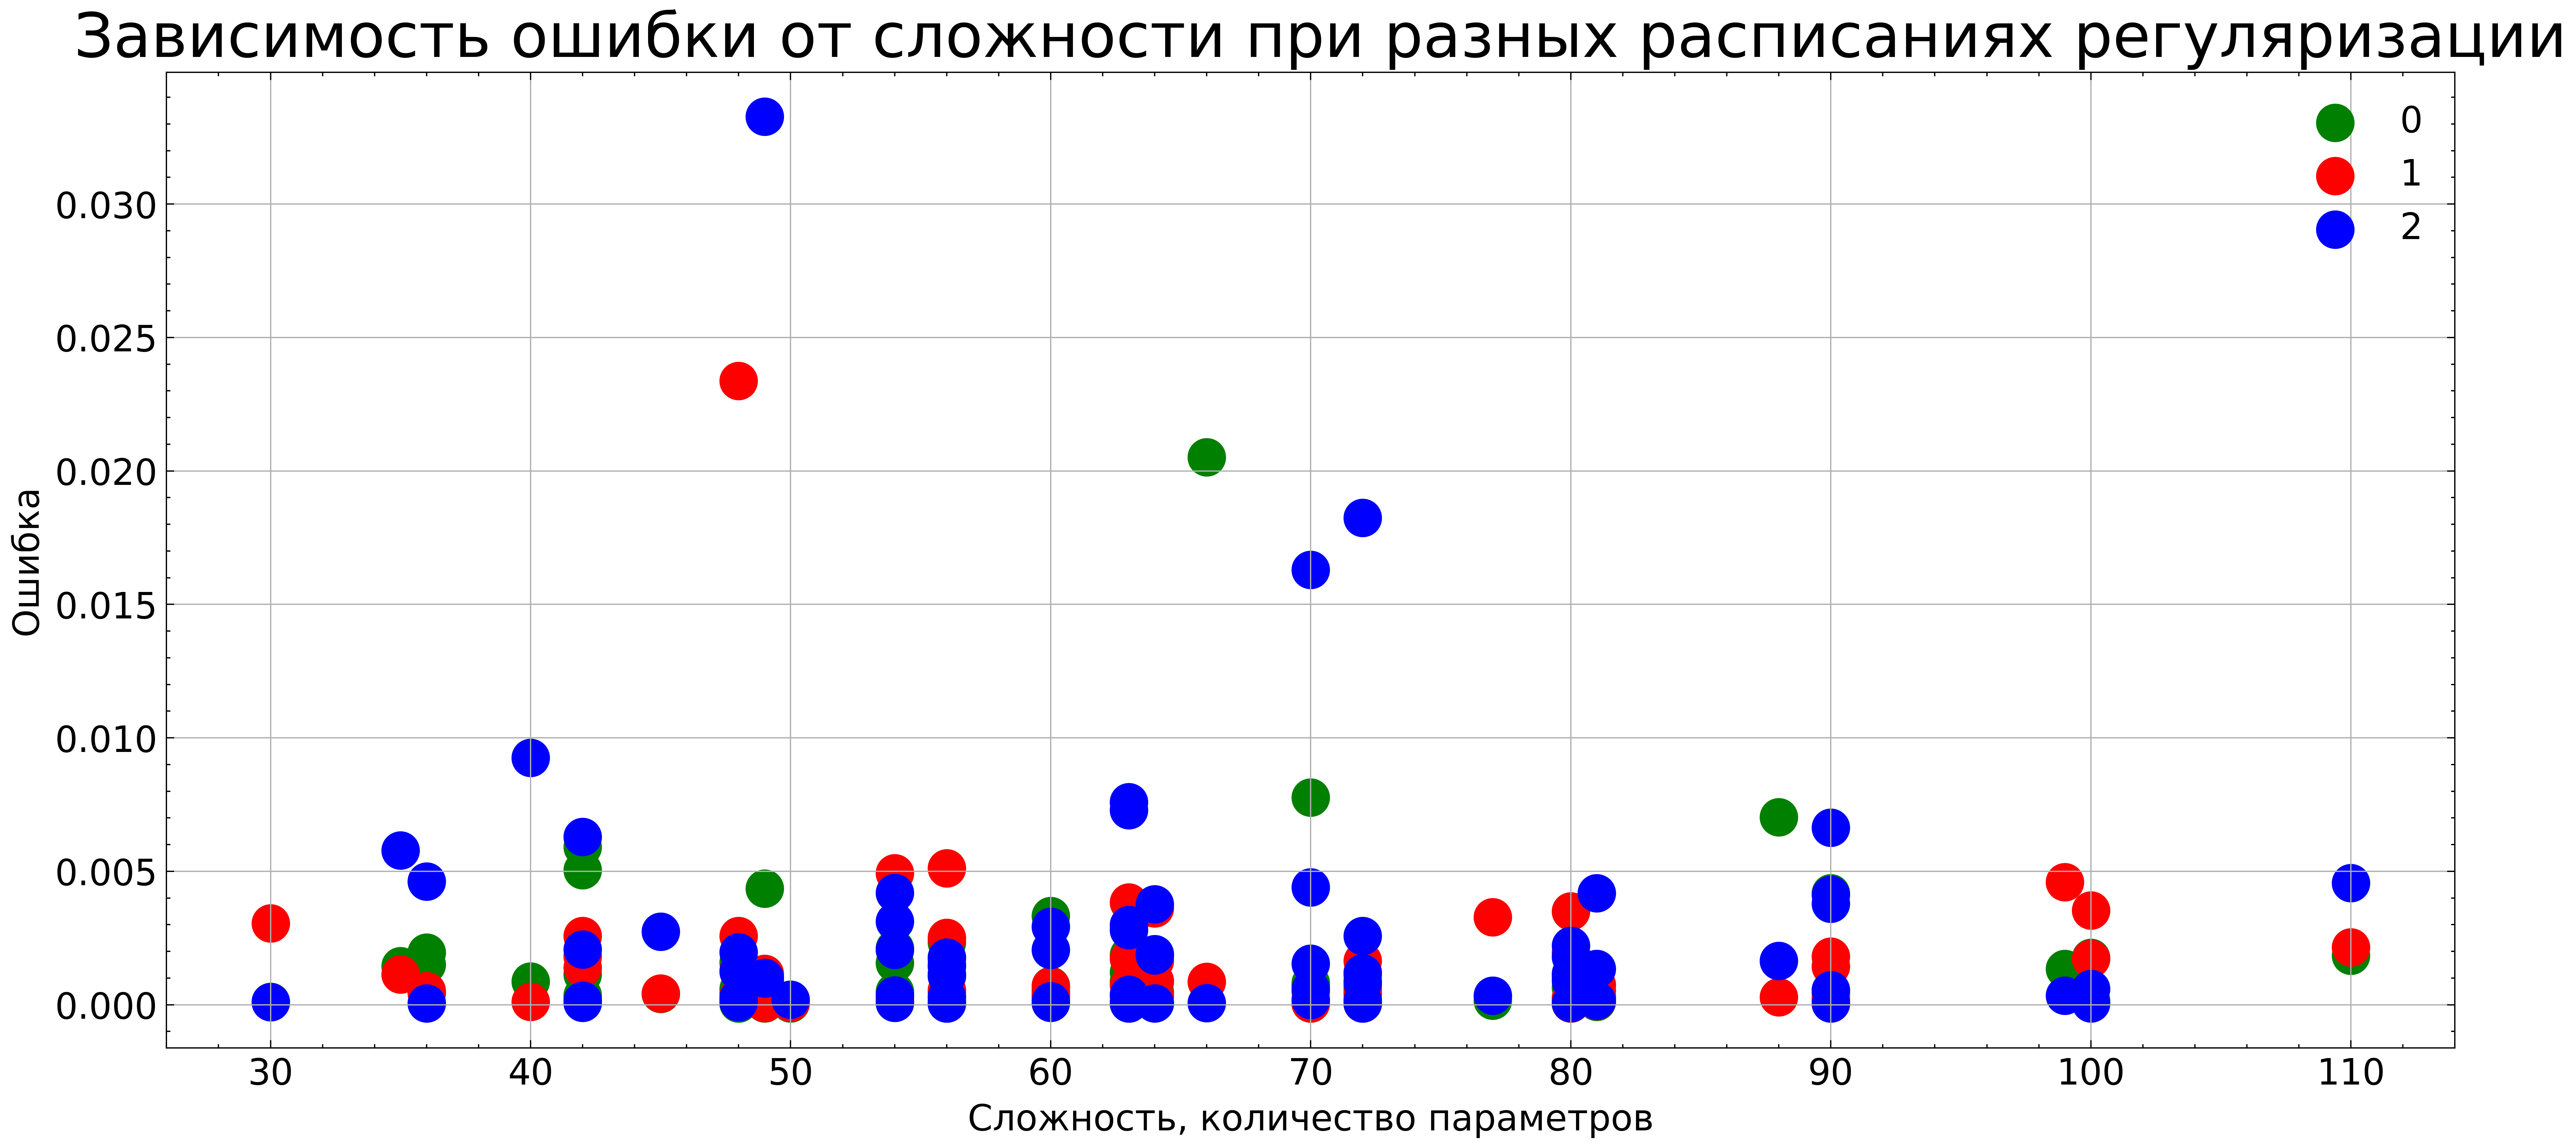
\includegraphics[width=\linewidth]{new_complexity.png}}

\label{fig:opt schedule 2}
\end{figure}
Зависимость между сложностью и точностью для разных расписаний оптимизации.
\end{center}
\end{frame}
%----------------------------------------------------------------------------------------------------------
\begin{frame}{Зависимость между устойчивостью и сложностью}
\begin{center}
\begin{figure}[h!]
\center{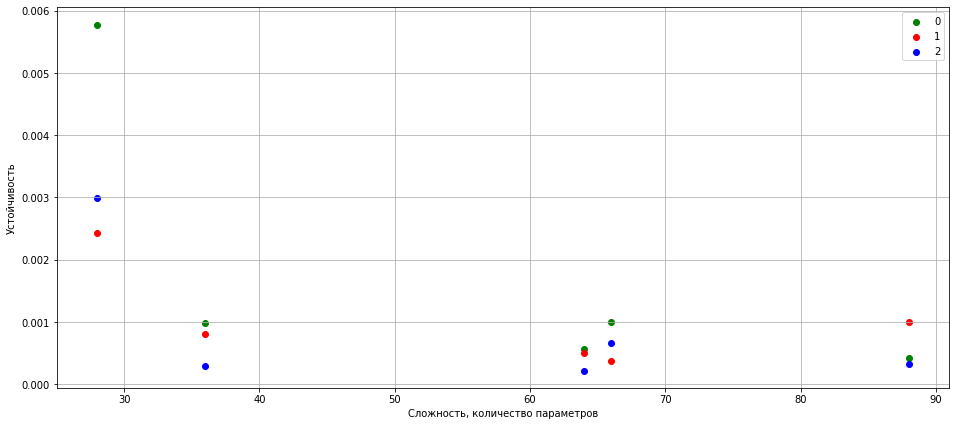
\includegraphics[width=\linewidth]{stability.png}}
\label{fig:opt schedule 2}
\end{figure}
Зависимость между сложностью и устойчивостью для разных расписаний оптимизации.
\end{center}
\end{frame}

%----------------------------------------------------------------------------------------------------------
\begin{frame}{Заключение}

    \begin{enumerate}
           \item 
        Показано, что регуляризованная модель имеет большую точность при равной сложности.
        \item 
        Показано, что регуляризованная модель имеет лучшую устойчивость при равной сложности.
        \item 
        Это предварительные результаты, по окончательным будет построена таблица с сравнением точности, сложности и устойчивости по разным выборкам и конфигурациям модели.
    \end{enumerate}
% Список литературы:
% \begin{thebibliography}{1}
			
% 			\bibitem{1}
% 			\BibAuthor{Tikhonov, Andrey N and Arsenin, Vasiliy Y}
% 			\BibTitle{Solutions of ill-posed problems}~//
% 			\BibJournal{New York, 1977}
			
% 			\bibitem{journals/corr/HaDL16}
% 			\BibAuthor{Svens{\'e}n, Markus and Bishop, Christopher M}
% 			\BibTitle{Pattern Recognition and Machine Learning}
			
% 			\bibitem{author09anyscience}
% 			\BibAuthor{Tibshirani, Robert}
% 			\BibTitle{Regression shrinkage and selection via the lasso}~//
% 			\BibJournal{Journal of the Royal Statistical Society: Series B (Methodological), 1966}
			
			
% 		\end{thebibliography}

\end{frame}
\end{document} 


%----------------------------------------------------------------------------------------------------------
\begin{frame}{Пример расписания регуляризации}
Первый вариант :
\begin{enumerate}
    \item[Шаг 1]
    Первые $s$ слоев обучаются как автокодировщик, а последние $k - s$ слоев обучаются как нейронная сеть. На второй итерации веса автокодировщика замораживаются и больше не оптимизируются.
    \item[Шаг 2]
    В функцию ошибки добавляются все регуляризаторы $s+1$-ого слоя кроме автокодировщика. Сеть дообучается. Веса $s+1$ слоя замораживаются, процедура идет дальше: к $s+2$-ому слою добавляются все регуляризаторы кроме автокодировщика с параметрами 1, сеть дообучается и так далее.
\end{enumerate}

\end{frame}
%----------------------------------------------------------------------------------------------------------
\begin{frame}{Пример расписания регуляризации}
Второй вариант :
\begin{enumerate}
    \item[Шаг 1]
    Первые $s$ слоев обучаются как автокодировщик, а последние $k - s$ слоев обучаются как нейронная сеть. На второй итерации веса автокодировщика замораживаются и больше не оптимизируются.
    \item[Шаг 2]
    Начиная с $s+1$ в функцию ошибки добавляется новый регуляризатор ко всем слоям, сеть дообучается, веса на $s+1$ слое замораживаются. Процедура продолжается далее, с каждой новой итерацией добавляется новый регуляризатор ко всем слоям, начиная с последнего замороженного.
\end{enumerate}

\end{frame}
